\chapter{Scale setting}%\addcontentsline{toc}{chapter}{Scale setting}

%%%%%%%%%%%%%%%%%%%%%%%%%%%%%%%%%%%%%%%%%%%%%%%%%%%%%%%%%%%
%%%%%%%%%%%%%%%%%%%%%%%%%%%%%%%%%%%%%%%%%%%%%%%%%%%%%%%%%%%
%%%%%%%%%%%%%%%%%%%%%%%%%%%%%%%%%%%%%%%%%%%%%%%%%%%%%%%%%%%
%%%%%%%%%%%%%%%%%%%%%%%%%%%%%%%%%%%%%%%%%%%%%%%%%%%%%%%%%%%

\label{ch_ss}

%%%%%%%%%%%%%%%%%%%%%%%%%%%%%%%%%%%%%%%%%%%%%%%%%%%%%%%%%%%
%%%%%%%%%%%%%%%%%%%%%%%%%%%%%%%%%%%%%%%%%%%%%%%%%%%%%%%%%%%
%%%%%%%%%%%%%%%%%%%%%%%%%%%%%%%%%%%%%%%%%%%%%%%%%%%%%%%%%%%
%%%%%%%%%%%%%%%%%%%%%%%%%%%%%%%%%%%%%%%%%%%%%%%%%%%%%%%%%%%

\section{Motivation}
\label{ch_ss:sec:introduction}

The scale setting involves the precise determination of one reference observable, the scale, in physical units, to which any other observable is compared in order to extract the value of the latter in physical units. 

We will use the gradient flow scale $t_0$ introduced in Sec.~\ref{ch_observables:sec:Flow} as an intermediate reference scale since it can be computed on the lattice with high precision. Following the discussion in Sec.~\ref{ch_foundation:sec:ss}, we choose for the phenomenological input the linear combination of the decay constants of the pion and kaon~\citep{Bruno:2016plf}
\begin{equation}
\label{ch_ss:eq:fpik}
\Lambda\equiv f_{\pi K}=\frac{2}{3}\left(f_K+\frac{1}{2}f_{\pi}\right).
\end{equation}
After measuring $\sqrt{t_0}f_{\pi K}$ for each ensemble, one must perform a chiral-continuum extrapolation in order to extract its value at physical values of the quark masses and in the continuum. To define the physical point we use the pion and kaon physical masses, or equivalently the dimensionless quantities $\phi_2$ and $\phi_4$ in eqs.~(\ref{ch_ma:eq:phi2}-\ref{ch_ma:eq:phi4}). Thanks to the mass shifting procedure in Sec.~\ref{ch_ma:sec:chiral_traj}, the value of $\phi_4$ is kept fixed to its physical value along our trajectory in the quark mass plane, and as a result the chiral extrapolation needs to be done in $\phi_2$ only. For the determination of the physical value of the latter we employ the iterative procedure explained at the end of Sec. \ref{ch_ma:sec:chiral_traj}. The latter relies on the physical input in eq.~(\ref{ch_ss:eq:isoQCD}) and an educated guess for the physical value of $t_0$, which is updated at each iterative step with the new determination of $t_0^{\textrm{ph}}$ coming from the scale setting analysis. Thus, with each iterative step both the values of $\phi_2$ to which we perform the chiral extrapolation and the value of $\phi_4$ to which we shift our observables are updated until convergence in $t_0^{\textrm{ph}}$ is obtained, which happens after a few iterative steps.

We employ an $\mathcal{O}(a)$ improved lattice action. Furthermore, in the calculation of $\sqrt{8t_0}f_{\pi K}$ we  employ the relevant improvement coefficients to remove $\mathcal{O}(a)$ lattice artifacts for the Wilson unitary setup. On the other hand, in the mixed action setup, we employ all known improvement coefficients in addition to relying on the $\mathcal{O}(a)$ improvement mechanism at maximal twist. Therefore, we expect lattice artifacts to start at $\mathcal{O}(a^2)$ for $\sqrt{t_0}f_{\pi K}$.

In order to perform the chiral-continuum limit, we explore different ways of parameterizing the dependence on $\phi_2$ ($\phi_4$ is constant thanks to the mass shifting procedure of Sec.~\ref{ch_ma:sec:chiral_traj}) and on the lattice spacing $a$, and employ the model averaging techniques introduced in Sec.~\ref{ch_observables:sec:MA}.

After performing the chiral-continuum limit, using as external physical input the values of the pion and kaon decay constants we can determine the value of the scale $t_0$ as
\begin{equation}
\sqrt{t_0^{\textrm{ph}}}=\frac{\left.\left(\sqrt{t_0}f_{\pi K}\right)^{\textrm{latt}}\right|_
{\phi_2^{\textrm{ph}},\;a=0}}{f_{\pi K}^{\textrm{exp}}}.
\end{equation}

Specifically, we consider ensembles with $N_f=2+1$ dynamical quarks, and thus assume isospin symmetry for the up and down flavors. Since we work in the limit of isosymmetric QCD (isoQCD), in which electromagnetic and strong isospin corrections are not explicitly included, we need to use a prescription to define the physical inputs in this limit. We opt for the values proposed in~\citep{FlavourLatticeAveragingGroupFLAG:2021npn}
\begin{gather}
\label{ch_ss:eq:isoQCD}
m_{\pi}^{\textrm{isoQCD}}=134.9768(5)\;{\textrm{MeV}}, \quad
m_{K}^{\textrm{isoQCD}}=497.611(13)\;{\textrm{MeV}}, \\
\label{ch_ss:eq:isoQCD_fpi}
f_{\pi}^{\textrm{isoQCD}}=130.56(2)_{\textrm{exp}}(13)_{\textrm{QED}}(2)_{|V_{ud}|}\;{\textrm{MeV}}, \quad \\
\label{ch_ss:eq:isoQCD_fk}
f_{K}^{\textrm{isoQCD}}=157.2(2)_{\textrm{exp}}(2)_{\textrm{QED}}(4)_{|V_{us}|}\;{\textrm{MeV}}.
\end{gather} 
The kaon decay constant receives a large contribution to its uncertainty from the determination of the $|V_{us}|$ CKM matrix element. QED corrections are also more significant in the kaon decay constant as compared to the pion case. Although not relying on the kaon decay constant seems a desirable option, controlling the systematic uncertainties of the chiral-continuum extrapolation of $f_{\pi}$ is  at present more challenging than that of $f_K$. 

%%%%%%%%%%%%%%%%%%%%%%%%%%%%%%%%%%%%%%%%%%%%%%%%%%%%%%%%%%%
%%%%%%%%%%%%%%%%%%%%%%%%%%%%%%%%%%%%%%%%%%%%%%%%%%%%%%%%%%%
%%%%%%%%%%%%%%%%%%%%%%%%%%%%%%%%%%%%%%%%%%%%%%%%%%%%%%%%%%%
%%%%%%%%%%%%%%%%%%%%%%%%%%%%%%%%%%%%%%%%%%%%%%%%%%%%%%%%%%%


\section{Determination of $\sqrt{t_0}$ at the physical point}
\label{ch_ss:sec:Results}

The choice of the combination of decay constants $f_{\pi K}$ in eq.~(\ref{ch_ss:eq:fpik}) to set the scale is motivated by its chiral behavior, since at fixed value of $\phi_4$ its next-to-leading order (NLO) $SU(3)$ ChPT expression only depends on $\phi_2$ through chiral logarithms. To this order we have, using $m_u=m_d\equiv m_l$~\citep{FLAG16,Bar:2013ora}
\begin{align}
\label{ch_ss:eq:t0_chiral}
t_0&=t_{0,\textrm{ch}}\left(1+k_1\frac{2m_K^2+m_{\pi}^2}{(4\pi f)^2}\right), \\
f_{\pi}&=f\left[1+\frac{16B_0L_5}{f^2}m_l+\frac{16B_0L_4}{f^2}(2m_l+m_s)-2L(m_{\pi}^2)\right. \notag \\
&\left.-L(m_K^2)\right], \\
f_K&=f\left[1+\frac{8B_0L_5}{f^2}(m_l+m_s)+\frac{16B_0L_4}{f^2}(2m_l+m_s)\right. \notag \\
&\left.-\frac{3}{4}L(m_{\pi}^2)-\frac{3}{2}L(m_K^2)-\frac{3}{4}L(m_{\eta}^2)\right],
\end{align}
where $L(x)$ are chiral logarithms, defined as
\begin{equation}
L(x)=\frac{x}{(4\pi f)^2}\textrm{log}\frac{x}{(4\pi f)^2},
\end{equation}
and $f,t_{0,\textrm{ch}},k_1,B_0,L_i$ are low energy constants (LECs). The quark masses can be related to meson masses using the LO expressions
\begin{align}
m_{\pi}^2&=2B_0m_l, \\
m_K^2&=B_0(m_l+m_s), \\
m_{\eta}^2&=\frac{4}{3}m_K^2-\frac{1}{3}m_{\pi}^2.
\end{align}
This way, the combination $\sqrt{8t_0}f_{\pi K}$ reads
\begin{align}
\label{ch_ss:eq:SU3ChPT}
F_{\chi SU(3),\pi K}^{\textrm{cont}}(\phi_2)&\equiv\left(\sqrt{8t_0}f_{\pi K}\right)^{\textrm{cont}}= \notag \\
&=\frac{A}{4\pi}\left[1-\frac{7}{6}\tilde{L}\left(\frac{\phi_2}{A^2}\right)-\frac{4}{3}\tilde{L}\left(\frac{\phi_4-\frac{1}{2}\phi_2}{A^2}\right)\right. \notag \\
&\left.-\frac{1}{2}\tilde{L}\left(\frac{\frac{4}{3}\phi_4-\phi_2}{A^2}\right)+\frac{B}{A^2}\phi_4\right],
\end{align}
with modified chiral logarithms given by
\begin{equation}
\label{ch_ss:eq:log}
\tilde{L}(x)=x{\textrm{log}}\left(x\right),
\end{equation}
and where we absorbed the LECs into the definition of the parameters $A,B$ as
\begin{align}
A&=4\pi\sqrt{8t_{0,\textrm{ch}}}f, \\
B&=\frac{(16\pi)^2}{3}(L_5+3L_4)+k_1.
\end{align} 
We use the expression in eq.~(\ref{ch_ss:eq:SU3ChPT}) to perform the chiral-continuum extrapolation of $\sqrt{8t_0}f_{\pi K}$. We will use the label $[SU(3)\chi PT]$ for this continuum mass-dependence. 

To probe the systematic effects associated with chiral extrapolation, in addition to the $SU(3)$ ChPT expressions, we also consider $SU(2)$ formulae in which the mass dependence of the strange quark is absorbed 
in the corresponding LECs. The expressions at NLO reads~\citep{SU2}
\begin{align}
\label{ch_ss:eq:SU2fpi}
f_{\pi}&=f\left[1+\frac{8(2L_4+L_5)}{f^2}m_{\pi}^2-2L(m_{\pi}^2)\right], \\
\label{ch_ss:eq:SU2fk}
f_K&=f^{(K)}(m_s)\left[1+\frac{c(m_s)}{f^2}m_{\pi}^2-\frac{3}{4}L(m_{\pi}^2)\right].
\end{align}
More specifically, we either consider the case in which $f^{(K)}(m_s)$ and $c(m_s)$ follow a linear dependence on $m_s$ or in which they remain constant. Since in the expression of $f_{\pi}$ in eq.~(\ref{ch_ss:eq:SU2fpi}), the dependence on $m_s$ appears only through sea quark loop effects, we assume that the LECs $f$ and $L_{4,5}$ are independent of $m_s$. After some algebra, we arrive at
\begin{align}
\label{ch_ss:eq:SU2pik}
F_{\chi SU(2),\piK}^{\textrm{cont}}(\phi_2)&=B+C\phi_2+D\phi_4-E\tilde{L}\left(\frac{\phi_2}{A^2}\right),
\end{align}
With the fit parameters $A,B,C,D,E$ combinations of the LECs appearing in eqs.~(\ref{ch_ss:eq:SU2fpi}-\ref{ch_ss:eq:SU2fk}). Since we mass shifted to a constant value of $\phi_4$, the fit cannot distinguish between $B$ and $D\phi_4$, and we may group these two terms into a single term in order to reduce the number of fit parameters. A term of type $D\phi_4$ may arise from the chiral expansion of $t_0$ in eq.~(\ref{ch_ss:eq:t0_chiral}) even when $f^{(K)}(m_s)$ and $c(m_s)$ are considered to be independent of $m_s$.

Another possibility for the extrapolation to the physical point is to use Taylor expansions in $\phi_2$ around the symmetric point. We have considered Taylor expansions to the second and fourth order as follows
\begin{equation}
\label{ch_ss:eq:Tay}
F_{\textrm{Tay},\pi K}^{\textrm{cont}}(\phi_2)\equiv\sqrt{8t_0}f_{\pi K}^{\textrm{cont}}=A+B\left(\phi_2-\phi_2^{\textrm{sym}}\right)^2,
\end{equation}
or
\begin{equation}
\label{ch_ss:eq:Tay4}
F_{\textrm{Tay},\pi K}^{\textrm{cont}}(\phi_2)=A+B\left(\phi_2-\phi_2^{\textrm{sym}}\right)^2+C\left(\phi_2-\phi_2^{\textrm{sym}}\right)^4,
\end{equation}
labeling these models as $[Tay]$ and $[Tay4]$. Due to symmetry reasons~\citep{Bietenholz:2011qq}, there are no terms with odd powers of $\phi_2-\phi_2^{\textrm{sym}}$.

In addition to the extrapolation in the pion mass, we need to supplement these fit functions with cutoff effects in order to describe our lattice data. To this end, we will explore three possibilities
\begin{align}
\label{ch_ss:eq:a2}
F^{\textrm{latt}}(\phi_2)&=F^{\textrm{cont}}(\phi_2)+W\frac{a^2}{8t_0},\\
\label{ch_ss:eq:aas}
F^{\textrm{latt}}(\phi_2)&=F^{\textrm{cont}}(\phi_2)+W\frac{a^2}{8t_0}\alpha_S^{\Gamma}(a),\\
\label{ch_ss:eq:a2phi2}
F^{\textrm{latt}}(\phi_2)&=F^{\textrm{cont}}(\phi_2)+\left(W+Z\phi_2\right)\frac{a^2}{8t_0}.
\end{align}
We assign the labels $[a^2]$, $[a^2\alpha_S^{\Gamma}]$ and $[a^2+a^2\phi_2]$ to characterize the lattice artifacts of these models, respectively. The lattice artifact in eq.~(\ref{ch_ss:eq:aas}) is motivated by~\citep{Husung:2022kvi} where logarithmic corrections in the lattice spacing $a$ are analyzed. In particular, a set of possible powers $\Gamma_i$ are found to contribute. 

Since it is not feasible to include several independent fitting parameters to characterize these logarithmic corrections, we chose to include a single such term. We vary the choice of $\Gamma_i$ by monitoring its impact on the extracted value of $t_0^{\textrm{phys}}$ after averaging over the set of models. As $t_0^{\textrm{phys}}$ is observed to be independent of the choice of $\Gamma_i$, we restrict ourselves to the smallest value, $\Gamma_i=-0.111$, in the model average. 

The systematic uncertainty in the extraction of $\sqrt{t_0^{\textrm{ph}}}$ is assessed by the model variation using the TIC introduced in Sec.~\ref{ch_observables:sec:MA}. We vary over the different ways of performing the chiral-continuum limits introduced above, as well as over the possibility of performing data cuts. In particular, we consider the following cuts (in addition to the ``no cut'' choice)
\begin{align}
\label{ch_ss:eq:cuts}
\beta&>3.40, \\
\beta&>3.46, \\
m_{\pi}&<420\;\textrm{MeV}, \\
m_{\pi}&<350\;\textrm{MeV}, \\
\beta&>3.40\;\&\;\phi_2<0.6, \\
m_{\pi}L&>4.1,
\end{align}
meaning that for each cut we keep only ensembles satisfying the corresponding condition above. With these cut choices, we explore the systematic uncertainty associated with performing lattice simulations at coarse lattice spacings, pion masses significantly heavier than in Nature, and small volumes that may introduce finite volume effects.

In general, the models included in the model average correspond to good fits in terms of their p-values (see Tables~\ref{apex_ma:tab:w}-\ref{apex_ma:tab:comb}). This means that the TIC will tend to heavily penalize any cut in the data, since the lattice data can be well described by the fit functions explored without performing any cuts. As a result, we observe that data points with the coarsest value of lattice spacing and/or with heavier pion masses -- which tend to have smaller uncertainties than those closer to the continuum and the physical point -- strongly constrain the model selection based on the TIC. In addition, the systematic effects associated with, for instance, the removal of the coarsest lattice spacing or of heaviest pion mass data are not always satisfactorily explored in such a model averaging framework. We therefore wish to extend the model averaging approach to introduce information on the regime of parameters in which the effective theories involved in the chiral-continuum extrapolations are known to perform best. For the case of the Symanzik expansion, this corresponds to the regime of smaller values of the lattice spacing, while for chiral perturbation theory it corresponds to the smaller values of the pion mass. The idea~\citep{DallaBrida:2016kgh} is to supplement the weight matrix $\mathcal{W}$ appearing in the definition of the $\chi^2$ of the fit (see Appendix~\ref{apex_chisq}) with a systematic error penalization for small values of the inverse coupling $\beta$ and heavy pions, according to 
\begin{equation}
\label{ch_ss:eq:Wpenal}
\mathcal{W}_{ij}^{-1}=C_{ij}\times\sqrt{1+c_i^2/C_{ii}}\sqrt{1+c_j^2/C_{jj}},
\end{equation}
where $C_{ij}$ is the element of the covariance matrix of the lattice data of $\sqrt{8t_0}f_{\pi K}$ for the ensembles $i$ and $j$, and $c_i$ is a penalization factor given by
\begin{equation}
\label{ch_ss:eq:penal}
c_i^2=c_{\beta}^2\left(\frac{a^2}{8t_0}\right)^4+c_{\phi_2}^2\phi_2^4,
\end{equation}
which is motivated by the fact that at coarse lattice spacings we expect $\mathcal{O}(a^4)$ cutoff effects to be relevant, and for heavy pions we expect that higher order effects of $\mathcal{O}(m_{\pi}^4)$ in the chiral expansion could play a role. More specifically, the penalization in $\beta$ will only be applied in $\beta=3.40$ ensembles, while the penalization in $\phi_2$ acts only on symmetric point ensembles $\phi_2\sim0.73$. The coefficients $c_{\beta,\phi_2}$ in eq.~(\ref{ch_ss:eq:penal}) are chosen such that the elements of the weight matrix $\mathcal{W}$ appearing in the $\chi^2$ function (see Appendix~\ref{apex_chisq}) for ensembles at the symmetric point or at the coarsest lattice spacing, are no longer significantly enhanced with respect to those  lying closer to the continuum or at the physical pion mass. We remark that the determination of the expectation value of the $\chi^2$ allows to determine the p-value of a fit based on a generic weight matrix $\mathcal{W}$~\citep{Bruno:2022mfy} such as that in eq.~(\ref{ch_ss:eq:Wpenal}). As expected, in the presence of an additional term in the $\chi^2$ that suppresses the relative weights of the coarsest lattice spacing and the heaviest pion masses, we observe that the p-values of the fits without cuts are similar to those of the fits implementing the cuts $\beta>3.40$ and $m_{\pi}<420$ MeV. Moreover, the weights in the model average are more evenly distributed compared to the case in which we do not include systematic effects in the $\chi^2$ function. Setting any of the $c_{\beta,\phi_2}$ coefficients to infinity is equivalent to performing the cut $\beta>3.40$ or $m_{\pi}<420$ MeV, while setting them to zero corresponds to the absence of cut.

As anticipated, we will carry out the chiral-continuum extrapolations using two sets of lattice data: the Wilson unitary setup and the mixed action. Universality arguments imply that the two regularizations should approach a common continuum limit value with different lattice artifacts. We can thus perform the continuum-chiral extrapolations for the Wilson data, for the mixed action, or for a combined data set, parameterizing the data with the same continuum limit mass-dependence $F^{\textrm{cont}}(\phi_2)$ but different cutoff effects (parameterized by different $W,Z$ fit parameters for Wilson and mixed action data). We observe that by combining the Wilson and mixed action calculations, an increase in statistical precision and in the control of the continuum limit extrapolation of $\sqrt{8t_0}f_{\pi K}$ can be achieved. As a universality check, we performed the continuum limit extrapolation of the Wilson and mixed action determinations of $\sqrt{8t_0}f_{\pi K}$ using only symmetric point ensembles, without imposing a common value in the continuum. Since all these points have the same value of $\phi_2$, they follow a line of constant physics as we approach towards the continuum limit. The extrapolation shown in Fig.~\ref{ch_ss:fig:universality} shows that both data sets agree perfectly well in the continuum. For this quantity, the mixed action data appears to receive milder discretization effects

Once the various models to extrapolate to the continuum and physical point have been explored, we use the model averaging technique introduced in Sec.~\ref{ch_observables:sec:MA} to assign a normalized weight to each model 
\begin{equation}
\label{ch_ss:eq:W}
W\propto\exp\left(-\frac{1}{2}\left(\chi^2-2\left<\chi^2\right>\right)\right),
\end{equation}
that allows us to compute a weighted average for $\sqrt{t_0^{\textrm{ph}}}$, as well as the associated systematic uncertainty
\begin{align}
\left<\sqrt{t_0^{\textrm{ph}}}\right>&=\sum_i\sqrt{t_0^{\textrm{ph,}(i)}}W^{(i)},\\
\sigma^2_{\textrm{syst}}&=\left<\sqrt{{t_0^{\textrm{ph}}}^2}\right>-\left<\sqrt{t_0^{\textrm{ph}}}\right>^2.
\end{align}

In Figs.~\ref{ch_ss:fig:BMA_w}-\ref{ch_ss:fig:BMA_comb} we show the model average results for the Wilson unitary setup, for the mixed action and for the combined analysis. In Appendix~\ref{apex_model_av_t0} we show the numerical results of $\sqrt{t_0^{\textrm{ph}}}$ for each model considered, together with their weights and p-values, for the Wilson, mixed action and combined analysis. In Fig.~\ref{ch_ss:fig:SU3a2} we show the pion mass dependence of the continuum-chiral extrapolation for model $[SU(3)\chi PT][a^2]$ and the combined data set (no cuts), together with the lattice spacing dependence for the same model, projecting all points to the physical pion mass $\phi_2^{\textrm{ph}}$ using the fit result for the continuum dependence $F^{\textrm{cont}}(\phi_2)$.

The results for $\sqrt{t_0^{\textrm{ph}}}$ in physical units as computed from the model average for the different data sets, using $f_{\pi K}^{\textrm{isoQCD}}$ as physical input, are
\begin{align}
\label{ch_ss:eq:t0ph_w}
\sqrt{t_0^{\textrm{ph}}}&=0.1433(9)_{\textrm{stat}}(4)_{\textrm{syst}}\;\textrm{fm, Wilson}, \\
\label{ch_ss:eq:t0ph_tm}
\sqrt{t_0^{\textrm{ph}}}&=0.1442(10)_{\textrm{stat}}(4)_{\textrm{syst}}\;\textrm{fm, Mixed action}, \\
\label{ch_ss:eq:t0ph_c}
\sqrt{t_0^{\textrm{ph}}}&=0.1438(7)_{\textrm{stat}}(4)_{\textrm{syst}}\;\textrm{fm, Combined}.
\end{align}
We show a comparison of these results with other determinations in the literature using $N_f=2+1$ flavors of dynamical quarks in Fig.~\ref{ch_ss:fig:t0_compar}.

We tested the impact of varying over the choice of the coefficients $c_{\beta}$ and $c_{\phi_2}$ in eq.~(\ref{ch_ss:eq:penal}) and found that the central values of the physical value of $\sqrt{t_0}$ in eqs.~(\ref{ch_ss:eq:t0ph_w}-\ref{ch_ss:eq:t0ph_c}) move always well within $1\sigma$, and not a big impact in the final uncertainty is found. More specifically, for the Combined analysis case if one removes altogether the $\beta=3.40$ and $m_{\pi}=420$ MeV ensembles from the analysis, the statistical and systematic uncertainties found are the same as in eq.~(\ref{ch_ss:eq:t0ph_c}). Additionally, one finds a statistical uncertainty of $6\times10^{-4}$ fm and a systematic uncertainty of $3\times10^{-4}$ fm for the Combined analysis result by setting $c_{\beta}=c_{\phi_2}=0$ and including the $\beta=3.40$ and $m_{\pi}=420$ MeV ensembles into the analysis. Finally, we tested the impact of using~\citep{FLAG16} for the physical input of $m_{\pi},\;m_K,\;f_{\pi},\;f_K$ instead of using the input in~\citep{FlavourLatticeAveragingGroupFLAG:2021npn} quoted in eqs.~(\ref{ch_ss:eq:isoQCD}-\ref{ch_ss:eq:isoQCD_fk}). This comparison is shown in Fig.~\ref{ch_ss:fig:FLAG}.

The statistical uncertainty in eqs.~(\ref{ch_ss:eq:t0ph_w}-\ref{ch_ss:eq:t0ph_c}) stems from the gauge noise of the CLS configurations, the uncertainties in the renormalization constants and improvement coefficients in Tables~\ref{ch_observables:tab:Z}-\ref{ch_observables:tab:b}, and the physical inputs in eqs.~(\ref{ch_ss:eq:isoQCD}-\ref{ch_ss:eq:isoQCD_fk}). We show the splitting of these contributions for the combined analysis case in Table~\ref{ch_ss:tab:stat}.

\begin{longtable}{c c}
\label{ch_ss:tab:stat}
	Contributions to total error squared of $\sqrt{t_0}$ [Combined] & \\
	\toprule
	Model variation (systematic) & $25.42\%$ \\
	Gauge ensembles & $55.72\%$ \\
	Renormalization and improvement & $0.82\%$ \\
	$\left|V_{ud}\right|$ & $0.01\%$ \\
	$\left|V_{us}\right|$ & $11.7\%$ \\
	QED corrections to $f_{\pi}$ & $0.32\%$ \\
	QED corrections to $f_K$ & $3\%$ \\
	Experimental input for $f_{\pi}$ & $0.01\%$ \\
	Experimental input for $f_K$ & $3\%$ \\
	IsoQCD pion and kaon meson masses & $<0.01\%$ \\
    \bottomrule
    \caption{Different contributions to total uncertainty for $\sqrt{t_0}$ for the combined analysis of both Wilson and mixed action lattice data in eq.~(\ref{ch_ss:eq:t0ph_c}).}
\end{longtable}

\begin{figure}
    \centering
    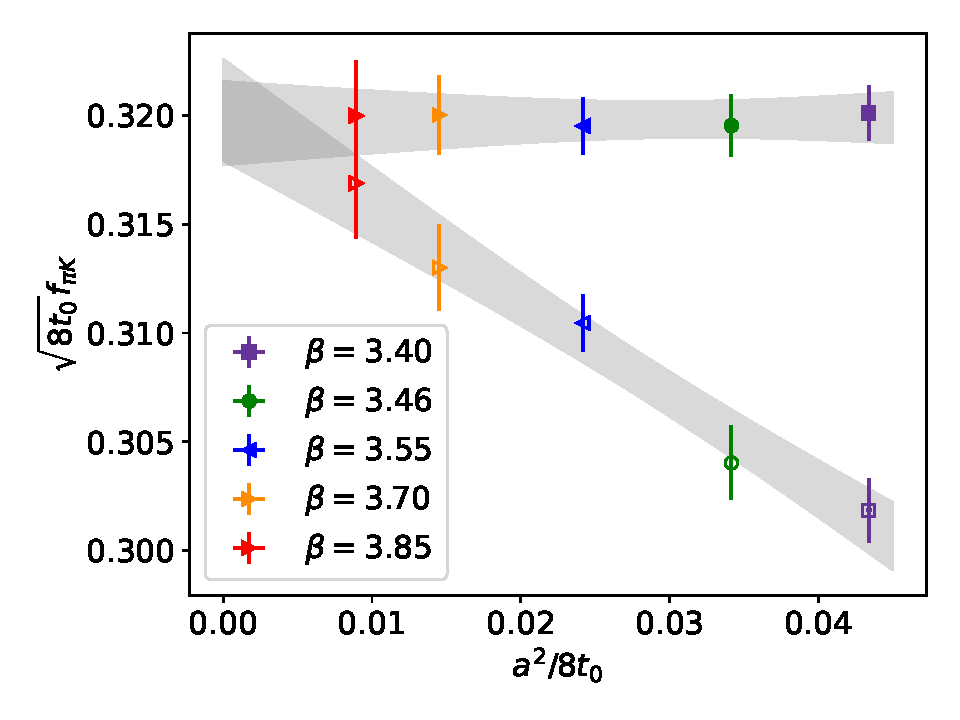
\includegraphics[width=1.\textwidth]{./cap5/figs/continuum_sym.pdf}
    \caption{Continuum limit extrapolation of symmetric point ensembles for the Wilson unitary results (empty points) and for the mixed action results (filled points). In order to perform a universality check and verify that both regularizations share the same continuum limit, a common result at vanishing lattice spacing is not imposed. Cutoff effects are parameterized as pure $\mathcal{O}(a^2)$ artifacts independent for each regularization.}
    \label{ch_ss:fig:universality}
\end{figure}

\begin{figure}
    \centering
    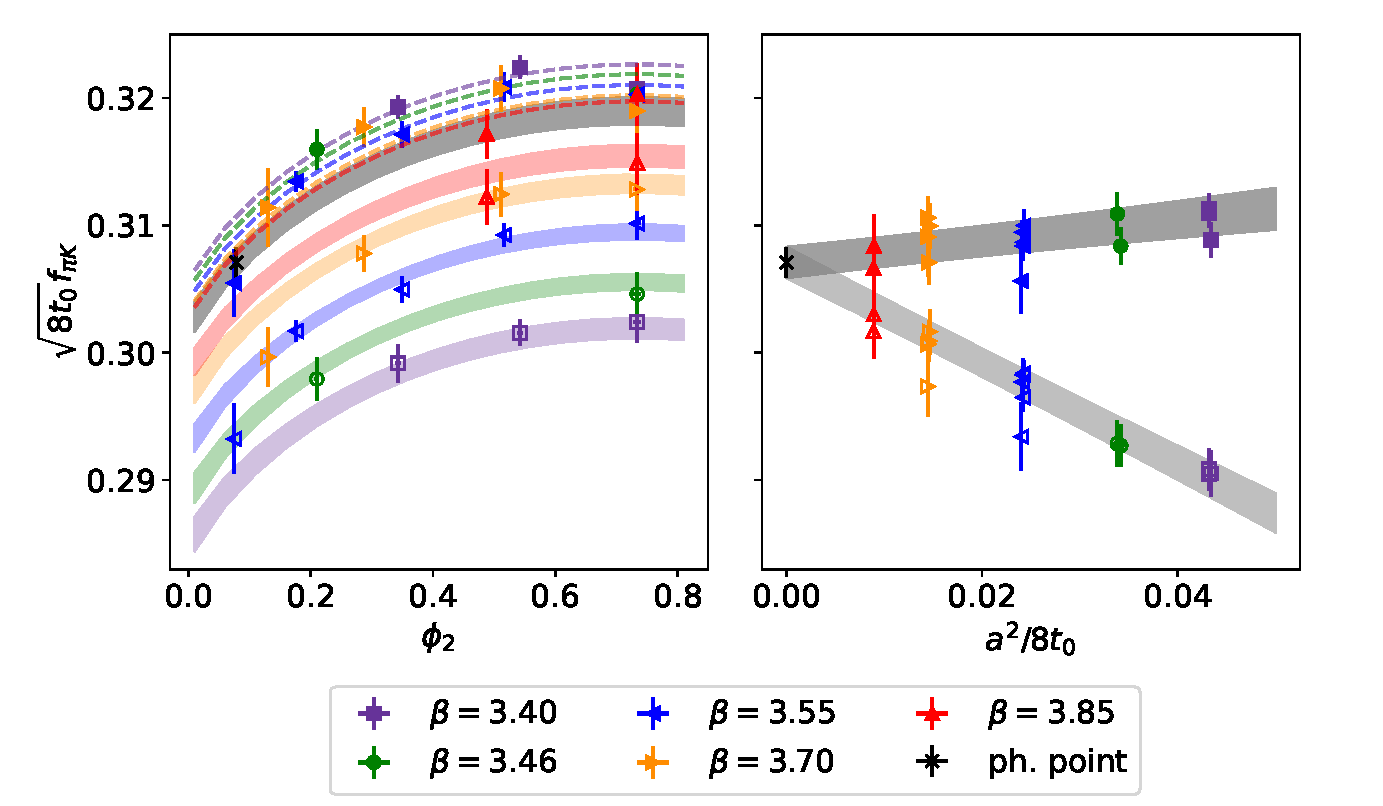
\includegraphics[width=1.\textwidth, angle=0]{./cap5/figs/SU3_comb.pdf}
    \caption{\textit{Top}: Light quark mass-dependence of $\sqrt{8t_0}f_{\pi K}$ for the $SU(3)$ ChPT model with pure $\mathcal{O}(a^2)$ cutoff effects and absence of cuts in data, corresponding to the label: $[SU(3)\chi PT][a^2][-]$. We show the result of the combined fit of both Wilson (empty) and mixed action (filled) results. The colored bands represent the pion mass dependence for each lattice spacing for the Wilson results, while the dashed lines represent the dependence for the mixed action results. In the latter case we only plot the central value of the corresponding bands for visualization purposes. \textit{Bottom}: the same model, with points projected to the physical pion mass $\phi_2^{\textrm{ph}}$ using the fit result for the continuum mass dependence $F(\phi_2)^{\textrm{cont}}$. In this plot we show the lattice spacing dependence of our ensembles. The  additional systematic effect terms in the $\chi^2$ (see eq.~(\ref{ch_ss:eq:penal})) were included. The p-value of this fit is $0.5532$.}
    \label{ch_ss:fig:SU3a2}
\end{figure}

\begin{figure}
    \centering
    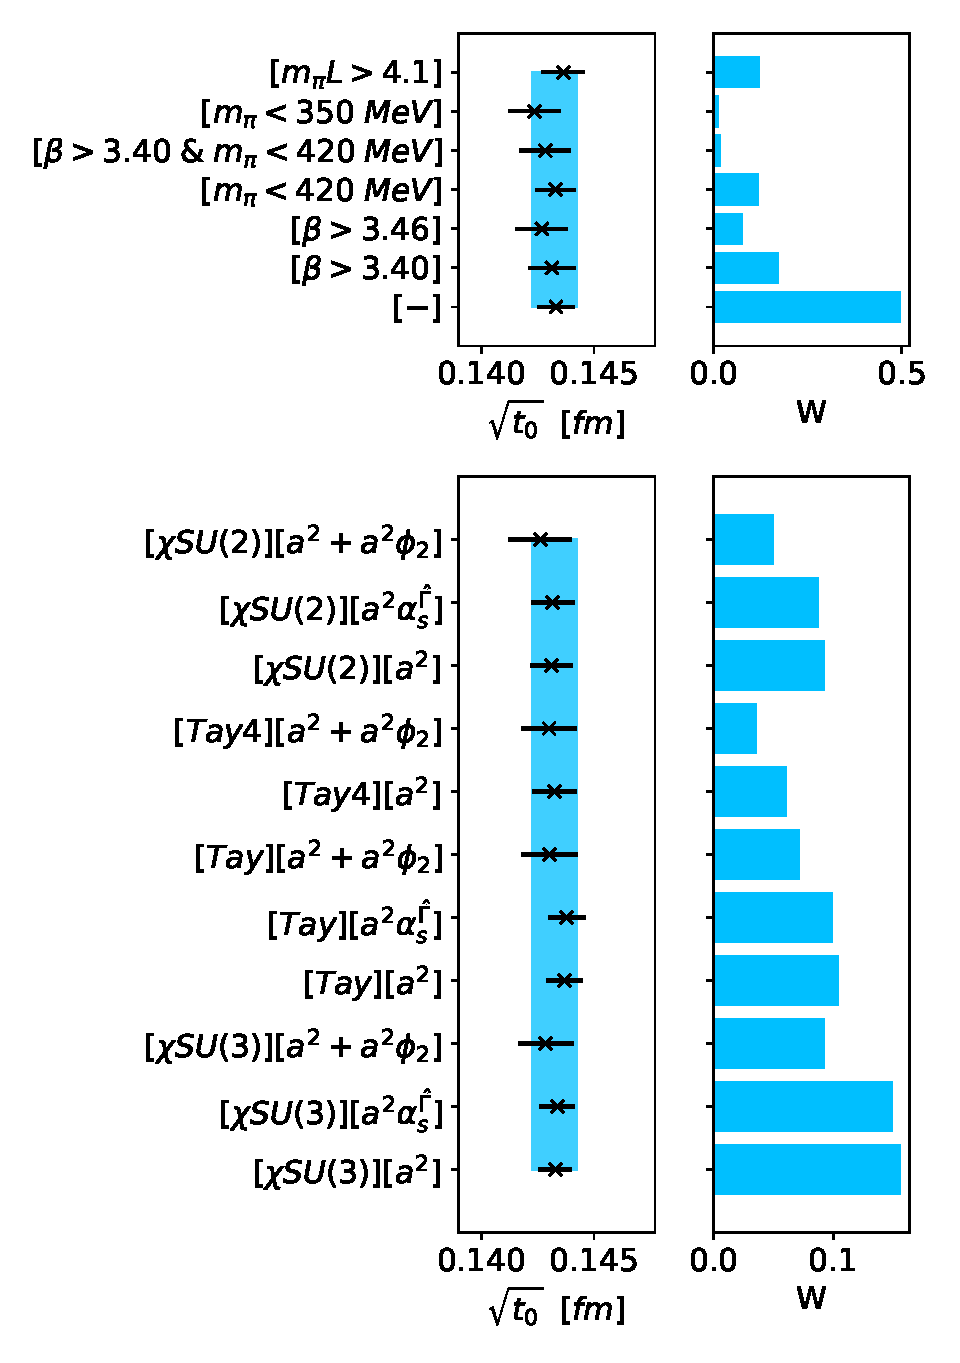
\includegraphics[width=1.\textwidth]{./cap5/figs/BMA_w_subav_c=1_cphi=0.0035.pdf}
    \caption{Model average results for the determination of $\sqrt{t_0}$ at the physical point based only on Wilson lattice data and $f_{\pi K}$ as physical input. \textit{Top}: model average over cuts in the data, the model weight defined in eq.~(\ref{ch_ss:eq:W}). For each label of the cut performed to the data displayed in the panel, an average according to the model weights was taken over the various fit forms employed to perform the chiral-continuum extrapolation. The label ``[-]'' refers to the case in which no cuts are applied to the data. In all models the penalization of eq.~(\ref{ch_ss:eq:penal}) was included, so even in the ``[-]'' models points at $\beta=3.40$ and $m_{\pi}=420$ MeV are penalized in the fit. \textit{Bottom}: model average over different fit forms employed in  the chiral-continuum extrapolation. For each label of the fit form displayed in the panel, an average was taken over the various data cuts according to the model weights. The blue vertical band shows the result of the model average over the full set of considered models with systematic and statistical uncertainties added in quadrature. We provide Tables connecting each label to the corresponding fit models in Appendix~\ref{apex_model_av_t0}, as well as results of $\sqrt{t_0}$, model weight and p-value for each individual model.}
    \label{ch_ss:fig:BMA_w}
\end{figure}

\begin{figure}
    \centering
    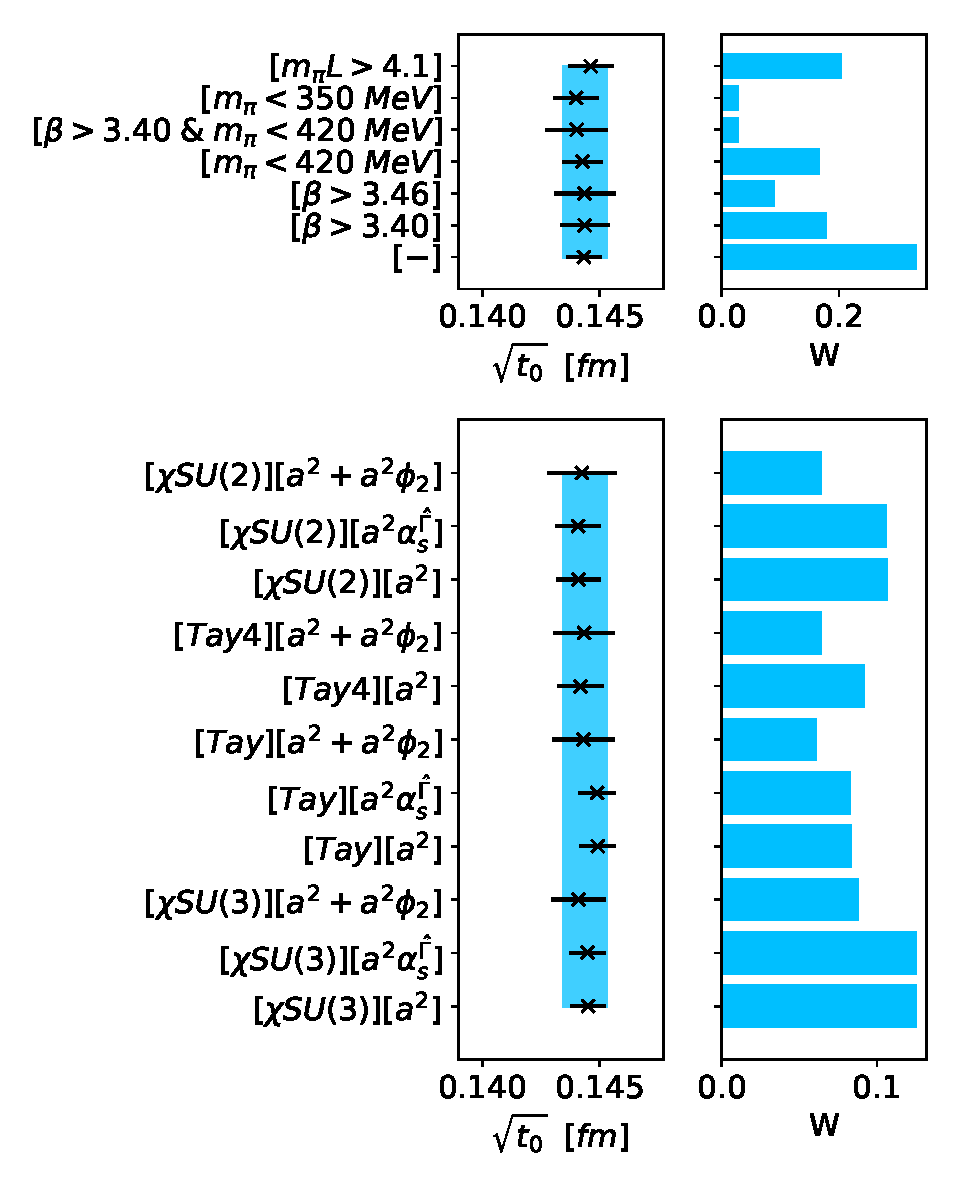
\includegraphics[width=1.\textwidth]{./cap5/figs/BMA_tm_subav_c=1_cphi=0.0035.pdf}
    \caption{Model average results for the determination of $\sqrt{t_0}$ at the physical point based only on mixed action lattice data and $f_{\pi K}$ as physical input. \textit{Top}: model average over cuts in the data, the model weight defined in eq.~(\ref{ch_ss:eq:W}). For each label of the cut performed to the data displayed in the panel, an average according to the model weights was taken over the various fit forms employed to perform the chiral-continuum extrapolation. The label ``[-]'' refers to the case in which no cuts are applied to the data. In all models the penalization of eq.~(\ref{ch_ss:eq:penal}) was included, so even in the ``[-]'' models points at $\beta=3.40$ and $m_{\pi}=420$ MeV are penalized in the fit. \textit{Bottom}: model average over different fit forms employed in  the chiral-continuum extrapolation. For each label of the fit form displayed in the panel, an average was taken over the various data cuts according to the model weights. The blue vertical band shows the result of the model average over the full set of considered models with systematic and statistical uncertainties added in quadrature. We provide Tables connecting each label to the corresponding fit models in Appendix~\ref{apex_model_av_t0}, as well as results of $\sqrt{t_0}$, model weight and p-value for each individual model.}
    \label{ch_ss:fig:BMA_tm}
\end{figure}

\begin{figure}
    \centering
    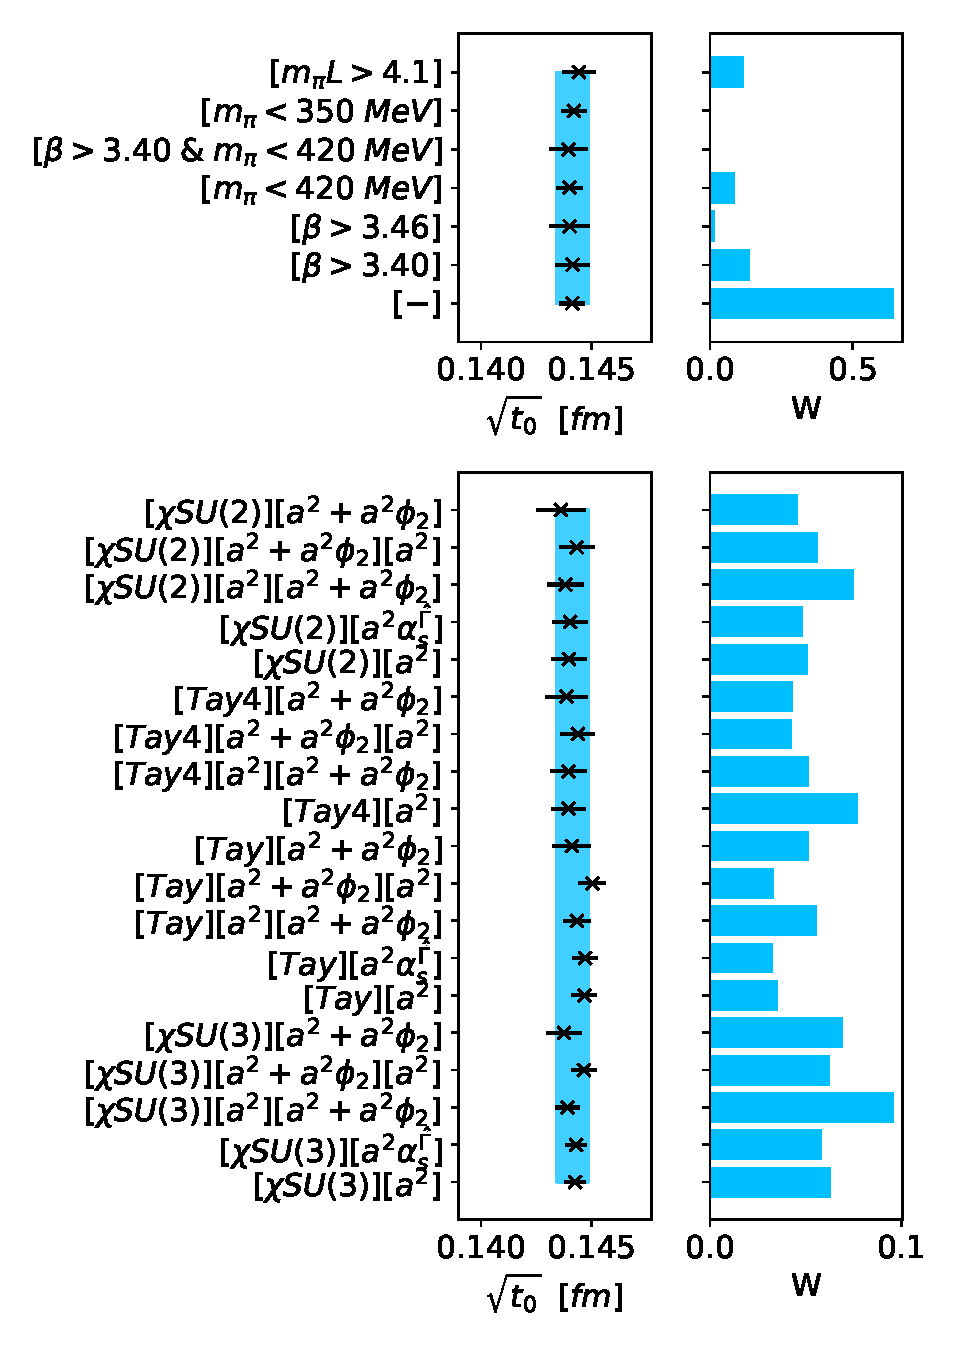
\includegraphics[width=1.\textwidth]{./cap5/figs/BMA_comb_subav_c=1_cphi=0.0035.pdf}
    \caption{Model average results for the determination of $\sqrt{t_0}$ at the physical point based on the combination of Wilson and mixed action lattice data and $f_{\pi K}$ as physical input. \textit{Top}: model average over cuts in the data, the model weight defined in eq.~(\ref{ch_ss:eq:W}). For each label of the cut performed to the data displayed in the panel, an average according to the model weights was taken over the various fit forms employed to perform the chiral-continuum extrapolation. The label ``[-]'' refers to the case in which no cuts are applied to the data. In all models the penalization of eq.~(\ref{ch_ss:eq:penal}) was included, so even in the ``[-]'' models points at $\beta=3.40$ and $m_{\pi}=420$ MeV are penalized in the fit. \textit{Bottom}: model average over different fit forms employed in  the chiral-continuum extrapolation. For each label of the fit form displayed in the panel, an average was taken over the various data cuts according to the model weights. The blue vertical band shows the result of the model average over the full set of considered models with systematic and statistical uncertainties added in quadrature. We provide Tables connecting each label to the corresponding fit models in Appendix~\ref{apex_model_av_t0}, as well as results of $\sqrt{t_0}$, model weight and p-value for each individual model.}
    \label{ch_ss:fig:BMA_comb}
\end{figure}

\begin{figure}
    \centering
    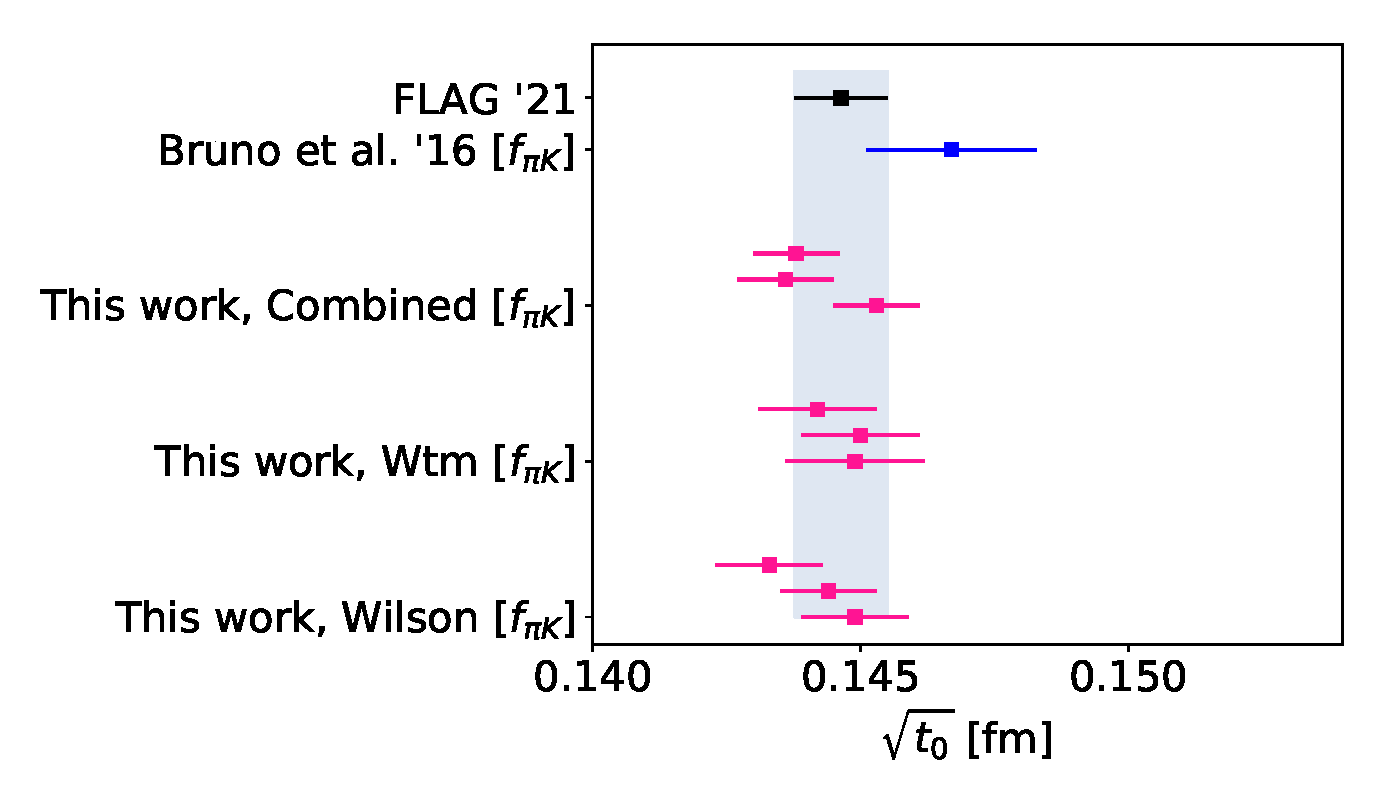
\includegraphics[width=1.\textwidth]{./cap5/figs/t0_compar_FLAG.pdf}
    \caption{Comparison of our determination of $\sqrt{t_0}$ at the physical point with Bruno et al. `16~\citep{Bruno:2016plf}. For our determination, in each label of the panel we show three variations, from top to bottom: using the complete set of ensembles listed in Table~\ref{apex_ensembles:tab:ens}, with physical input from~\citep{FlavourLatticeAveragingGroupFLAG:2021npn} quoted in eqs.~(\ref{ch_ss:eq:isoQCD}-\ref{ch_ss:eq:isoQCD_fk}), and the systematic term in eq.~(\ref{ch_ss:eq:Wpenal}) added when doing the model average (results quoted in eqs.~(\ref{ch_ss:eq:t0ph_w})-\ref{ch_ss:eq:t0ph_c}); using the complete set of ensembles but removing the systematic term in eq.~(\ref{ch_ss:eq:Wpenal}) from the analysis, and using physical input from~\citep{FLAG16}; and using the set of ensembles that is common between the ones listed in Table~\ref{apex_ensembles:tab:ens} and the ones in~\citep{Bruno:2016plf}, without the systematic term in eq.~(\ref{ch_ss:eq:Wpenal}), and using physical input from~\citep{FLAG16}. The latest variation corresponds to an analysis following what was done in Bruno et al.~\citep{Bruno:2016plf}, and we observe an upwards drift of the central values in $\sqrt{t_0}$ in our results, approaching the determination of $\sqrt{t_0}$ in~\citep{Bruno:2016plf}. The remaining difference between our determination and that of~\citep{Bruno:2016plf} might be explained by our use of the model average technique and by the higher amount of statistics available for ensembles D200 and J303 with respect to~\citep{Bruno:2016plf}.}
    \label{ch_ss:fig:FLAG}
\end{figure}

\begin{figure}
    \centering
    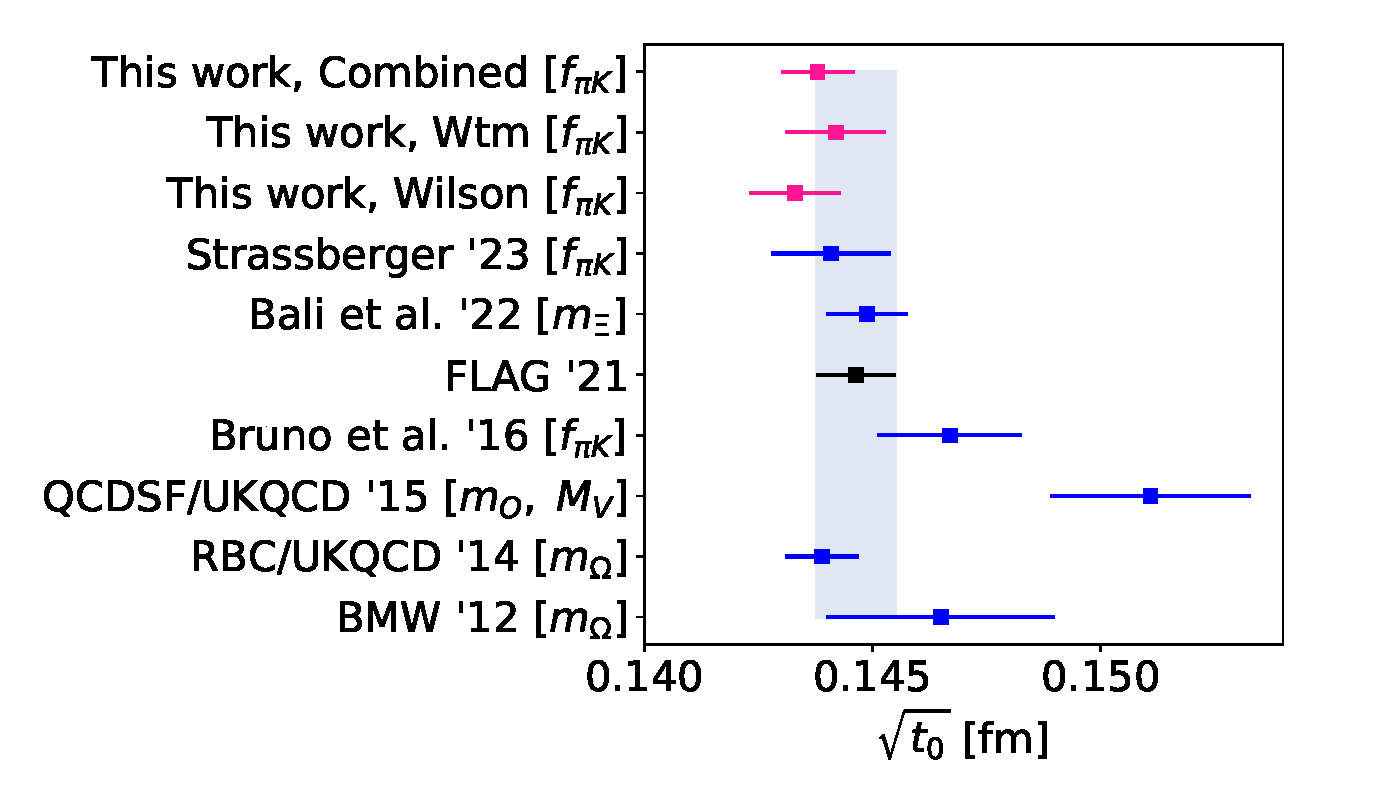
\includegraphics[width=1.\textwidth]{./cap5/figs/t0_compar.pdf}
    \caption{Comparison of our results in eqs.~(\ref{ch_ss:eq:t0ph_w}-\ref{ch_ss:eq:t0ph_c}) with other determinations of $\sqrt{t_0}$ in the literature using $N_f=2+1$ flavors of dynamical quarks. We specify between brackets the physical input used in each case to set the scale. BMW `12 refers to~\citep{BMW:2012hcm}. RBC/UKQCD `14 refers to \citep{UK14} and QCDSF/UKQCD `15 to~\citep{UK15}. Bruno et al. `16 refers to~\citep{Bruno:2016plf}, Bali et al. `22 to~\citep{RQCD_scale}, Strassberger `23 to~\citep{Strassberger:2023xnj}, and FLAG `21 to~\citep{FlavourLatticeAveragingGroupFLAG:2021npn}.}
    \label{ch_ss:fig:t0_compar}
\end{figure}

\section{Determination of $\sqrt{t_0}$ at the symmetric point}

The symmetric point is defined as the point in the quark mass plane at which the symmetric line defined by
\begin{equation}
m_{ud}\equiv m_l=m_s,
\end{equation}
and the chiral trajectory in eq.~(\ref{ch_ma:eq:chiral_traj}) intersect. In terms of our usual quantities $\phi_2,\phi_4$, the symmetric point satisfies
\begin{equation}
\phi_2=\frac{2}{3}\phi_4,
\end{equation}
where $\phi_4$ is given by its physical value after the iterative procedure to find $t_0^{\textrm{ph}}$ and after mass shifting (see Sec.~\ref{ch_ma:sec:chiral_traj}). In order to extract $t_0^{\textrm{sym}}=t_0(\phi_2^{\textrm{sym}},\phi_4^{\textrm{ph}})$, following~\citep{Strassberger:2023xnj} we build the ratio
\begin{equation}
\frac{\sqrt{t_0/a^2}}{\sqrt{t_0^{\textrm{sym}}/a^2}},
\end{equation}
where $\sqrt{t_0/a^2}$ is the measurement of the gradient flow scale in each ensemble while $\sqrt{t_0^{\textrm{sym}}/a^2}$ is the corresponding lattice determination, at the same value of the inverse coupling $\beta$, but using a symmetric point ensemble. Following~\citep{Strassberger:2023xnj} we fit this ratio to
\begin{equation}
\label{ch_ss:eq:fit_t0_sym}
F(\phi_2)=\sqrt{1+p(\phi_2-\phi_2^{\textrm{sym}})}.
\end{equation}
We find this fit form to properly describe the lattice data. More specifically, no lattice artifacts are discerned from fits with $\mathcal{O}(a^2)$, $\mathcal{O}(a^2\phi_2)$ and/or $\mathcal{O}(a^2\alpha_S^{\Gamma})$ cutoff effects. The result of this fit is shown in Fig.~\ref{ch_ss:fig:t0_sym}. Once the data is fitted, we extract $t_0^{\textrm{sym}}$ in physical units as
\begin{equation}
\sqrt{t_0^{\textrm{sym}}}=\frac{\sqrt{t_0^{\textrm{ph}}}}{F(\phi_2^{\textrm{ph}})}.
\end{equation}
For $t_0^{\textrm{ph}}$ and $\phi_2^{\textrm{ph}}$ we can use our determination for the Wilson, mixed action or combined data sets. The result for the scale at the symmetric point is, depending on this choice
\begin{align}
\label{ch_ss:eq:t0_sym}
\sqrt{t_0^{\textrm{sym}}}&=0.1429(9)_{\textrm{stat}}(4)_{\textrm{syst}}\;\textrm{fm, Wilson}, \\
\sqrt{t_0^{\textrm{sym}}}&=0.1439(10)_{\textrm{stat}}(4)_{\textrm{syst}}\;\textrm{fm, Mixed action}, \\
\sqrt{t_0^{\textrm{sym}}}&=0.1435(7)_{\textrm{stat}}(4)_{\textrm{syst}}\;\textrm{fm, Combined}.
\end{align}

\begin{figure}
    \centering
    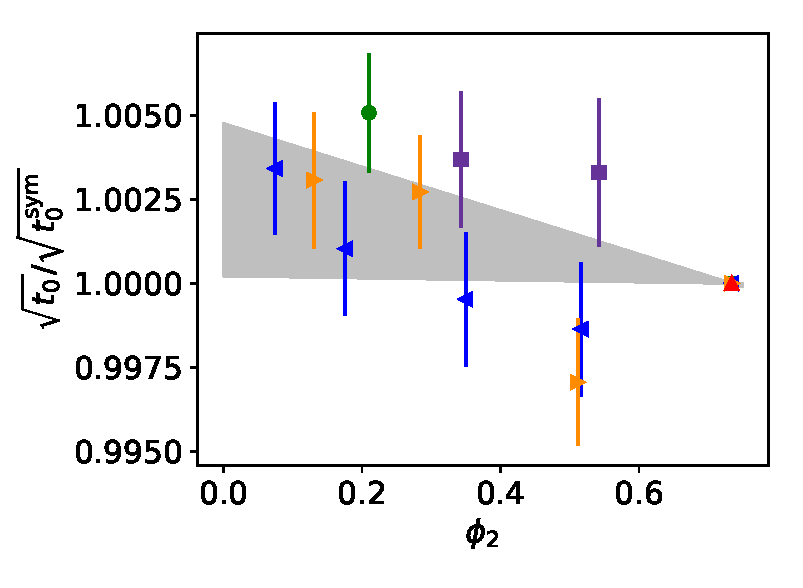
\includegraphics[width=1.\textwidth]{./cap5/figs/t0_sym.pdf}
    \caption{Fit to eq.~(\ref{ch_ss:eq:fit_t0_sym}) in order to extract $t_0$ at the symmetric point. }
    \label{ch_ss:fig:t0_sym}
\end{figure}

\section{Determination of the lattice spacing for CLS ensembles}
\label{ch_ss:sec:t0_sym}

Just as in the previous section, we can use the fit to $\frac{\sqrt{t_0/a^2}}{\sqrt{t_0^{\textrm{sym}}/a^2}}$ to compute 
\begin{equation}
\left(\sqrt{\frac{t_0}{a^2}}\right)^{\textrm{ph}}=\sqrt{\frac{t_0^{\textrm{sym}}}{a^2}}F(\phi_2^{\textrm{ph}}).
\end{equation}
Then, the lattice spacing is extracted as
\begin{equation}
\label{ch_ss:eq:a}
a=\frac{\sqrt{t_0^{\textrm{ph}}}}{\left(\sqrt{\frac{t_0}{a^2}}\right)^{\textrm{ph}}}.
\end{equation}
For $\phi_2^{\textrm{ph}}$ we can either use our determinations	 of $t_0^{\textrm{ph}}$ for the Wilson, mixed action or combined data sets. Results for the lattice spacing are shown in Table~\ref{ch_ss:tab:a}.

\begin{longtable}{c c c c}
\label{ch_ss:tab:a}
$\beta$ & $a$ [fm] Wilson & $a$ [fm] mixed action & $a$ [fm] combined \\
\toprule
$3.40$ & $0.0842(6)_{\textrm{stat}}(2)_{\textrm{syst}}$ & $0.0848(6)_{\textrm{stat}}(3)_{\textrm{syst}}$ & $0.0845(5)_{\textrm{stat}}(2)_{\textrm{syst}}$ \\
$3.46$ & $0.0747(5)_{\textrm{stat}}(2)_{\textrm{syst}}$ & $0.0752(5)_{\textrm{stat}}(2)_{\textrm{syst}}$ & $0.0750(4)_{\textrm{stat}}(2)_{\textrm{syst}}$ \\
$3.55$ & $0.0629(4)_{\textrm{stat}}(2)_{\textrm{syst}}$ & $0.0633(4)_{\textrm{stat}}(2)_{\textrm{syst}}$ & $0.0631(3)_{\textrm{stat}}(2)_{\textrm{syst}}$ \\
$3.70$ & $0.0488(3)_{\textrm{stat}}(1)_{\textrm{syst}}$ & $0.0491(3)_{\textrm{stat}}(2)_{\textrm{syst}}$ & $0.0490(3)_{\textrm{stat}}(1)_{\textrm{syst}}$ \\
$3.85$ & $0.0382(2)_{\textrm{stat}}(1)_{\textrm{syst}}$ & $0.0385(3)_{\textrm{stat}}(1)_{\textrm{syst}}$ & $0.0384(2)_{\textrm{stat}}(1)_{\textrm{syst}}$ \\
\bottomrule
\caption{Values of the lattice spacing $a$ in physical units extracted from the determination of the gradient flow scale $t_0$ with the Wilson, mixed action and combined analysis. The lattice spacing is extracted from measures of both $t_0$ at the physical and symmetric points using eq.~(\ref{ch_ss:eq:a}).}
\end{longtable}

\section{Determination of $t_0^*$}

Yet another point in the $(\phi_2,\phi_4)$ plane of interest corresponds to the reference point in~\citep{Bruno:2016plf}
\begin{gather}
\phi_4=1.11, \quad \phi_2=\frac{2}{3}\phi_4\equiv\phi_2^{\textrm{sym}}.
\end{gather}
The scale $t_0$ evaluated at this point is
\begin{equation}
t_0^*=t_0\left(\phi_2^{\textrm{sym}},\;\phi_4=1.11\right),
\end{equation}
and its ratio to $\sqrt{t_0^{\textrm{ph}}}$ enters in the computation of the strong coupling in~\citep{DallaBrida:2022eua}. To compute $t_0^{*}$, we repeat the analysis by mass shifting our ensembles to the value $\phi_4=1.11$ without error and compute the gradient flow scale at the symmetric point as explained in the Sec.~\ref{ch_ss:sec:t0_sym}.

The values we find for $\sqrt{t_0^*}$ in physical units for the Wilson, mixed action and combined cases are
\begin{align}
\label{ch_ss:eq:t0*}
\sqrt{t_0^*}&=0.1432(9)_{\textrm{stat}}(4)_{\textrm{syst}}\;\textrm{fm, Wilson}, \\
\sqrt{t_0^*}&=0.1439(9)_{\textrm{stat}}(4)_{\textrm{syst}}\;\textrm{fm, Mixed action}, \\
\sqrt{t_0^*}&=0.1436(7)_{\textrm{stat}}(4)_{\textrm{syst}}\;\textrm{fm, Combined}.
\end{align}

%%%%%%%%%%%%%%%%%%%%%%%%%%%%%%%%%%%%%%%%%%%%%%%%%%%%%%%%%%%
%%%%%%%%%%%%%%%%%%%%%%%%%%%%%%%%%%%%%%%%%%%%%%%%%%%%%%%%%%%
%%%%%%%%%%%%%%%%%%%%%%%%%%%%%%%%%%%%%%%%%%%%%%%%%%%%%%%%%%%
%%%%%%%%%%%%%%%%%%%%%%%%%%%%%%%%%%%%%%%%%%%%%%%%%%%%%%%%%%%
